\chapter{Hash Function \& MAC}

\begin{flushleft}
    Abbiamo visto che le configurazioni di sicurezza della crittografia simmetrica sono: \textbf{confidenzialità}, \textbf{integrità} e \textbf{autenticità}. Abbiamo anche definito che Alice e Bob condividono la conoscenza di un'unica chiave per la comunicazione. Con i \textit{block cipher} siamo riusciti a ottenere \textbf{confidenzialità}. 

    \medskip

    \textcolor{red}{\textbf{\textit{Integrity}}}: è possibili identificare dal ricevente di un messaggio se quel messaggio è stato modificato durante la trasmissione. Consideriamo una comunicazione tra Alice e Bob, dove il messaggio verrà inviato da Alice, prima di farlo verrà calcolato a \textbf{\textit{small-sized digest}} che rappresenta il dato. In questo modo qualunque modifica al dato o al \textbf{\textit{digest}} può essere verificata - in questo caso non c'è bisogno della chiave - $d = H(m)$ dove:
    \begin{itemize}[nosep]
        \item \textbf{d} è il \textit{digest} della funzione.
        \item \textbf{H} è una funziona che ritorna una sequenza di byte che rappresenta il dato.
        \item \textbf{m} è il messaggio.
    \end{itemize}
    Alice a quel punto invia a Bob $m || d$ in questo modo, Bob può ricalcolarsi $d' = H(m)$ e accettare il messaggio da Alice - quindi verificarne l'\textbf{integrità} - se e solo se $d == d'$.

    \medskip

    \textcolor{red}{\textbf{\textit{Authenticity Guarantess}}}: il destinatario del messaggio può controllare se il mittente è un mittente legittimo - ovvero qualcuno che ha accesso alla chiave segreta simmetrica - è possibile \textit{bindare} una qualche informazione (metadato) per rendere l'informazione identificativa, ma quasto è utile solamente nella crittografia asimmetrica.

    \begin{figure}[h]
        \centering
        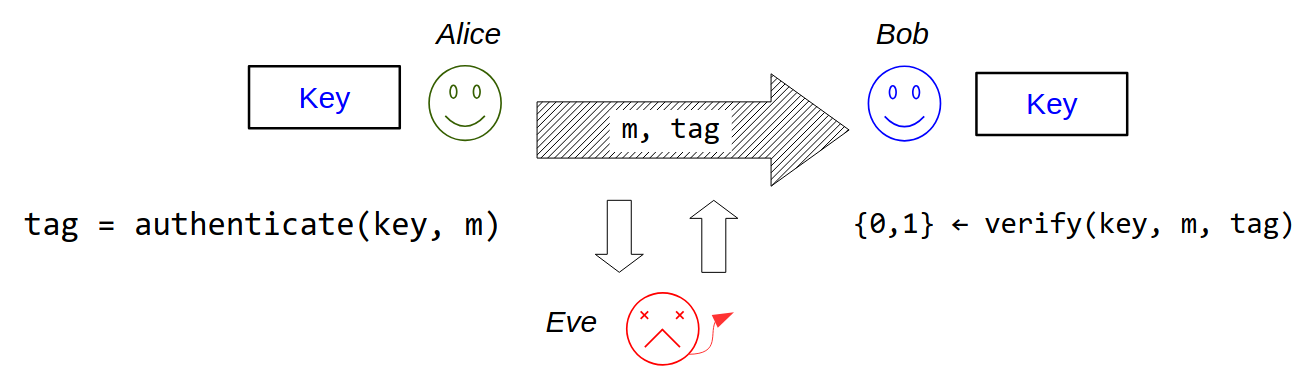
\includegraphics[width=0.55\textwidth]{img/mac_tag.png}
    \end{figure}

    L'integrità dell'informazione è condizione necessaria per l'autenticità, se l'attaccante può modificare il dato, allora può anche impersonificare il mittente del dato, violando l'autenticità.

    \smallskip

    È spesso confusa l'integrità del dato con la sua autenticità, nel contesto della sicurezza informatica noi cerchiamo l'autenticità - e quindi implicitamente l'integrità - per questo motivo andremo ad analizzare \textbf{\textit{authenticated encryption}}. È però fondamentale differenziare le due proprietà in quanto utilizzano schemi di crittografia differenti:
    \begin{itemize}[nosep]
        \item \textbf{\textit{Integrity}} utilizzo delle \textbf{funzioni hash}.
        \item \textbf{\textit{Authenticity}} utilizza i \textbf{\textit{Message Authentication Code - MAC}}, per ora andremo ad analizzarli nell'ambito della crittografia simmetrica.
    \end{itemize}

    \textcolor{red}{\textbf{\textit{Hash function \& cryptographic integrity guarantees}}} \\
    Andiamo, velocemente, ad analizzare quelle situazioni in cui è richiesta \textbf{\textit{integrità}} fuori dai requisiti di crittografia: come ad esempio modifiche al dato per errori di trasmissione o per guasti - normalmente scaturite da fenomeni fisici - per i quali sono presenti molteplici algoritmi, tra i quali: \textbf{\textit{parity}}, \textbf{CRC}, \textbf{\textit{checksum}}. In questo caso è possibile modellare la tipologia di attaccante come un \textbf{attaccante irrazionale} (perdita di bit randomici o a raffica). \\
    Nei settaggi di crittografia moderna, l'attaccante è sempre \textbf{razionale} e conosce gli \textbf{algoritmi crittografici} e si comporta di conseguenza, grazie al requisito di \textbf{\textit{cryptographic integrity-protection}} anche se noti i dati di base non deve essere capace di trovare una soluzione al problema nonostante l'assenza di una chiave condivisa. Anche in questo caso è presente la sicurezza computazione ma viene applicata in maniera differente.

\end{flushleft}

\section{Hash Function}

\begin{flushleft}

    \textcolor{red}{\textbf{Cryptography Hash Function}}: una funzione hash $H$ viene definita come: 

    {\centering
        $H : \{0, 1\}^* \mapsto \{0, 1\}^n$
    \par}

    ovvero è possibile mappare una quantità arbitraria di bit - nelle moderne funzioni hash $*$ è così ampio che può anche considerato a $\infty$ - in una sequenza fissata (piccola) - che è definita dall'algoritmo. L'ouput di $H$ viene chiamato \textbf{\textit{digest}} - le funzioni di hash esistono anche per scopi non prettamente crittografici. La dimensione di \textbf{n} è scelta in maniera tale che sia altamente improbabile che due input differenti generino lo stesso output, in questo modo il \textit{digest} è un informazione ``piccola'' che rappresenta univocamente l'informazione contenuto nel dato. È possibile paragonare il comportamento ad una \textbf{funzione di compressione pseudorandom}

    {\centering
        $m_1 \neq m_2 \longleftrightarrow d_1 \neq d_2$
    \par}

    Il comportamente delle funzioni hash - \textbf{PRF} - può essere applicato anche a circostante non crittografiche, ad esempio: \textbf{MD5} è una funzione hash deprecata, ma viene utilizzata per identificare in maniera univoca i commit su git. È possibile anche utilizzarle come \textbf{primitive} per costruire blocchi per altri schemi crittografici, ad esempio: alcuni \textbf{MAC} si basano su delle \textit{hash function} ed anche alcune \textbf{\textit{Key Derivation Function - KDF}}.

    \medskip

    In base al tipo di applicazione che stiamo utilizzando bisogna che la funzione hash sia resistente a diversi \textbf{\textit{attack model}}, tutti quanti, se no viene definita \textbf{deprecata}.

    \textcolor{red}{\textbf{\textit{Attack Models} Differenti}}
    \begin{center}
        \begin{minipage}[c]{0.75\textwidth}
            \begin{itemize}[nosep]
                \item \textbf{\textit{One Way}} anche nota come \textbf{\textit{first pre-image resistance}}, deve essere \textbf{efficiente} calcolare $H(m) = d$, ma \textbf{inefficiente} calcolare la funzione opposta, ovvero risalire a $m = H^{-1}(d)$
                \item \textbf{\textit{Second pre-image Collision Resistant}} ovvero dato un messaggio $m_1$ è \textbf{inefficiente} trovare un messaggio $m_2$ tale che $H(m_1) = H(m_2)$
                \item \textbf{\textit{Collision Resistant}} è \textbf{inefficiente} trovare una coppia di messaggi - \textbf{arbitrari} - $m_1$ e $m_2$ tale che $H(m_1) = H(m_2)$
            \end{itemize}
        \end{minipage}
        \hfill
        \begin{minipage}[c]{0.1\textwidth}
            \centering
            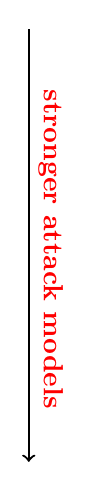
\begin{tikzpicture}[scale=1]
                \node[rotate=270, anchor=south, text=red] at (0,2.2) {\textbf{stronger attack models}};
                \draw[<-, thick, black] (0,-0.5) -- (0,5.0);
            \end{tikzpicture}
        \end{minipage}
    \end{center}

    \textcolor{red}{\textbf{\textit{First pre-Image Resistance}}}: dato un \textit{digest}, calcolarsi il dato. È tipicamente associato a \textbf{garanzie di confidenzialità} - può essere applicato a schemi di \textbf{KDF}.

    \begin{figure}[h]
        \centering
        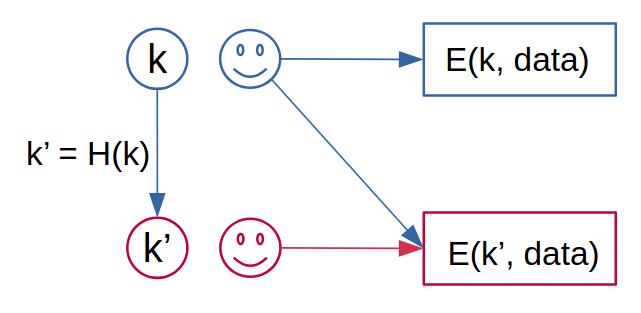
\includegraphics[width=0.45\textwidth]{img/one_way.png}
    \end{figure}
    
    Dato in input una chiave, ottengo in output un'altra chiave $k' = H(k)$ in questo caso cosa dovrebbe rompere Eve per riuscire a decifrare? In questo contesto anche se $H$ \textbf{non} è \textit{collision resistance} non è di interesse infatti anche se si trovasse un $k'' \; \text{t.c.} \; k' = H(k'') \rightarrow k \neq k''$ e quindi Eve non riuscirebbe a rompere lo schema crittografico di cifratura, l'unico modo per Eve di ottenere il dato in chiaro è riuscire a trovare una funzione $H^{-1} \; \text{t.c.} \; k = H^{-1}(k')$ e utilizzarla per decifrare le informazioni di Alice - ci basta: \textbf{\textit{One Way}}. \\
    L'unica limitazione è che se l'input $k$ è debole e quindi vulnerabile a \textit{brute-force} allora sarebbe possibile eseguire una ricerca esaustiva nell'insieme delle chiavi - \textbf{\textit{HKDF}}.

    \medskip

    \textcolor{red}{\textbf{\textit{Second pre-Image Collision Resistance}}}: dato un $d$ e un $m$ tale che $d = H(m)$ trovare un valore $m' \; \text{t.c.} \; d = H(m')$ è tecnicamente richiesta per gli \textbf{\textit{authentication schemes}} ad esempio nel contesto di \textbf{\textit{Keyed Hash Function}} - per l'offuscamento di password su DB - infatti riuscendo o a trovare $H^{-1}$ o trovando un'altro valore $m'$ che generi lo stesso \textit{digest} è possibile bypassare il controllo.
\end{flushleft}

\begin{boxA}
    \textcolor{orange}{\textbf{Esempio}}: \textbf{Download di dati}

    \medskip

    {\centering
        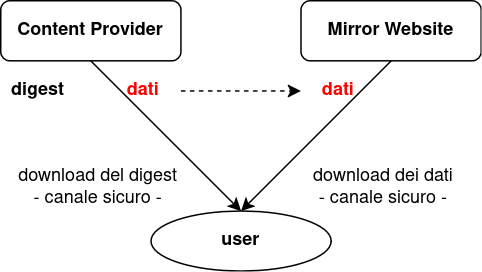
\includegraphics[width=0.45\textwidth]{img/hash_es.png}
    \par}

    Quando un sito mette a disposizione dei dati per il download - ad esempio un \textit{*.iso}, normalmente il contenuto per il download è disponibile su un \textit{server mirror}, quindi il \textit{provider} si calcola il \textit{digest} $d = H(m)$ e poi fa l'upload del contenuto sul \textit{server mirror}. L'utente si scarica il contenuto dal \textit{server mirror} e scarica il \textit{digest} dal \textit{provider}, successivamente calcola l'hash del dato scaricato $d_u = H(m_d)$ se e solo se $d_u = d$ accetta il dato scaricato.

    \smallskip

    In questo caso la funzione hash $H$ deve rispettare la ``normativa'' di sicurezza \textit{second pre-image collision resistance} in quanto il messaggio iniziale - la nostra \textit{*.iso} - viene fornita dal \textit{server mirror}. L'attaccante vincerebbe se riuscisse a trovare un messaggio $m_a \; \text{t.c.} \; H(m_d) = H(m_a)$ e contemporaneamente quel messaggio dovrebbe contenere un \textit{payload} malevolo. Solo in quel caso l'utente lo scaricherebbe il messaggio e la funzione di verifica - chiamata \textbf{\textit{verify}} - andrebbe a buon fine e quindi l'utente accetterebbe il nuovo messaggio.
\end{boxA}

\begin{flushleft}
    \textcolor{red}{\textbf{\textit{Collision Resistance}}}: riuscire ad ottenere, arbitrariamente, due messaggi $m_1$ e $m_2$ tali che $H(m_1) = H(m_2)$ è la più forte come garanzia di sicurezza, nel caso dovesse mancare, la funzione hash sarebbe molto facile da violare.
\end{flushleft}

\begin{boxA}
    \textcolor{orange}{\textbf{Esempio}}

    \medskip

    {\centering
        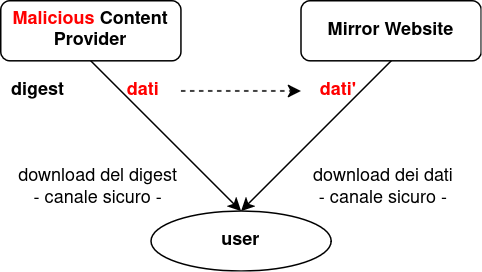
\includegraphics[width=0.45\textwidth]{img/hash_es_2.png}
    \par}

    Il \textit{provider} è malevolo e riesce a trovare due messaggio $m$ e $m'$ tali che $H(m) = H(m')$ a questo punto fa l'upload del messaggio malevolo sul \textit{server mirror}, l'utente che si scarica riesce a verificare la correttezza del \textit{digest}.
\end{boxA}

\begin{flushleft}
    \textcolor{red}{\textbf{\textit{Hash Function Security Parameters}}}: il \textbf{parametro di sicurezza} delle funzioni \textit{hash} è la \textbf{lunghezza del \textit{digest}} in quanto rappresenta le prossibili combinazioni di $n$ bit, ovvero i possibili valori prodotti dalla funzione \textit{hash} ($2^n$). Come discusso nel paragrafo di sicurezza computazionale, il valore di $n$ deve essere scelto considerando l'attacco noto più efficiente, analizzando anche il numero di operazioni richieste per trovare una collisione. 

    \smallskip

    Una funzione hash sicura è quello in cui l'attacco più efficiente per trovare una collisione è il \textbf{\textit{Birthday Attack}} che richiede $2^{n/2}$ ovvero la probabilità di trovare una collisione è del $50\%$ su $N$ ($\sqrt{N}$)

    \medskip

    Alcune delle più popolari funzioni hash:
    \begin{itemize}[nosep]
        \item \textbf{md5}: ad oggi deprecata, molto facile trovare delle collisioni.
        \item \textbf{sha1}: anche questa ad oggi deprecata, vi sono trovate delle collisioni. 160bit di \textit{digest}.
        \item \textbf{sha2}: sha1 ``potenziata'' ha diverse lunghezze del \textit{digest} in base alla versione: \textbf{sha224}, \textbf{sha256}, \textbf{sha384} e \textbf{sha512}.
        \item \textbf{sha3}: è stata implementata con una primitiva differente rispetto a sha1 e sha2, è stata standardizzata ufficialmente nel 2015, ha le stesse sottoversioni del sha2.
        \item \textbf{blake2}: utilizza come primitiva \textbf{chacha} non è ancora stata standardizzata dal NIST ma è molto popolari in certi ambienti, ad esempio, quello del \textit{software open source}.
    \end{itemize}

    Sia le funzioni \textbf{\textit{hash}} che le funzioni \textbf{\textit{mac}} vengono definite come funzioni con un solo input, ma è possibile concatenare più input, ma bisogna farlo in maniera sicura.

    {\centering
        $H('builtin' || 'security') = H('built' || 'insecurity') = H('builtinsecurity')$
    \par}

    Concatenare i risultati cercando di rendere univoco l'output:
    \begin{itemize}[nosep]
        \item utilizzando \textbf{caratteri speciali} per concatenare, se possibile: considersiamo che il carattere $;$ non sia ammesso come input allora sarà possibile concatenare gli input come: $d = H('builtin' \; || \; ';' \; || \; 'security')$
        \item \textbf{esplicitando} la \textbf{lunghezza dell'input}: $d = H('7buildinsecurity')$ 
    \end{itemize}
\end{flushleft}

\section{Message Authentication Code}

\begin{flushleft}
    Il destinatario può rilevare se il messaggio non è stato mandato da un mittente legittimo, che nel caso lo si andasse a definire all'interno della crittografia simmetrica, identificherebbe colui che conosce il segreto condiviso. Il \textbf{MAC} è una funzione che ha due input: la chiave e il message e come output un \textbf{\textit{tag}}.

    {\centering
        \textbf{tag} = \textbf{MAC}(\textit{key}, \textit{message})
    \par}

    La funzione \textbf{\textit{verify}} è simile a quella delle funzioni hash, ma include come input anche la chiave simmetrica.

    {\centering
        $\{0, 1\} \leftarrow$ \textbf{verify}(\textit{key}, \textit{message}, \textit{tag})
    \par}

    Il \textbf{MAC} permette a Bob di verificare che il messaggio è stato generato da Alice.
\end{flushleft}

\begin{flushleft}
    \textcolor{red}{\textbf{\textit{Attack Models for MAC}}}

    \medskip

    \begin{minipage}[c]{0.45\textwidth}
        \centering
        \textbf{\textit{Existential Forgery for Passive Eavesdropper}} \\
        L'attaccante osserva coppie $(m_i, t_i)$ trasmesse tra gli attori benevoli (Alice e Bob) ed è capace di \textit{forgiare} una nuova coppia $(m', t')$ mai inviata e l'attacco ha successo nel caso in cui il messaggio venga accettato.

        \smallskip

        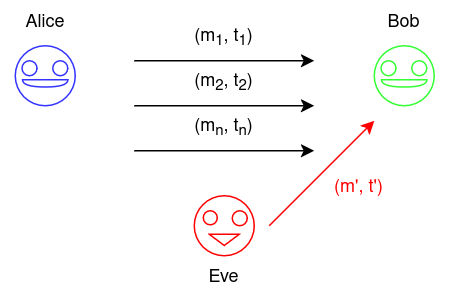
\includegraphics[width=\textwidth]{img/mac_am_1.png}
    \end{minipage}
    \hfill
    \begin{minipage}[c]{0.45\textwidth}
        \centering
        \textbf{\textit{Existential Forgery for Chosen Message}} \\
        In questo caso l'attaccante controlla i messaggi che vengono autenticati, quindi sceglie $n$ volte un messaggio $m_i$ e osserva il tag generato $t_i$ a quel punto se riesce a generare una nuova coppia $(m', t')$ non ancora inviata che verrà accettata l'attacco avrà avuto successo.

        \smallskip

        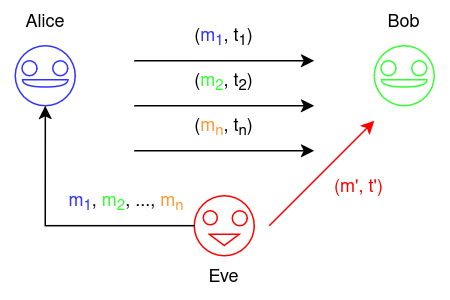
\includegraphics[width=\textwidth]{img/mac_am_2.png}
    \end{minipage}

    \smallskip

    \textcolor{red}{\textbf{\textit{MAC: Security Parameters}}}:
    \begin{itemize}[nosep]
        \item la \textbf{lunghezza della chiave}: l'attacco più efficiente deve essere quello di \textit{brute force}.
        \item la \textbf{lunghezza del \textit{tag}}: permette di determinare la dimensione del dato o il numero di messaggi autenticabili con la stessa chiave (dipende dal tipo di \textbf{\textit{MAC scheme}} che si vuole utilizzare). Ricordiamo che il \textit{tag} è \textbf{\textit{overhead}} sul messaggio e quindi è possibile minimizzarlo ma aggiungendo a livello di protocollo altri fattori di sicurezza. 
    \end{itemize}

    La scelta del \textbf{MAC} dipende dai requisiti nei quali va applicato. Disponibilità software (presenza di librerie), disponibilità hardware (accelleratore hardware) e l'abilità di soddisfare requisiti degli schemi (creare \textit{nonce}). Ogni tipologia di \textbf{MAC} offre un diverso \textit{trade-offs} in termini di: lunghezza e numero di messaggi, modelli di attacco e lunghezza del tag consentita.

    \medskip

    Consideriamo i \textbf{MAC} all'interno di una situazione di \textcolor{red}{\textbf{\textit{Replay Attack}}}. Abbiamo detto che il \textbf{MAC} può garantire che il \textit{tag} sia stato creato con una certa \textbf{chiave simmetrica}, ma nel contesto in cui siamo Eve re-invia lo stesso messaggio che ha inviato Alice a Bob, che è valido, perché creato da Alice - se Alice e Bob fossero due banchieri e Alice inviasse un messaggio con scritto "Aggiungi 1000 euro nell'account di Carlo". Con queste tipologie di attacco utilizzando la crittografia è difficile arginarle, è possibile però metterci una ``pezza'' lato architetturale (a livello \textbf{trasporto} o \textbf{applicazione}) ad esempio aggiungendo un \textbf{contatore univoco} al messaggio:
    
    {\centering
        \textbf{m} = (id=n, data), tag
    \par}

    Se consideriamo che la comunicazione sia \textit{full-duplex} - \textbf{\textit{Reflection Attacks}} - la possibilità che il messaggio venga inviato al mittente dello stessa e che venga verificato il \textit{tag} non è nulla, quindi si è aggiunto un bit di direzione del messaggio:

    {\centering
        \textbf{m} = (id=n, dir=val, data), tag
    \par}

    Il bit di direzione è aggiunto come \textbf{metadato} per un verifica ulteriore da parte del destinatario. È anche possibile utilizzare una difesa diversa, gestire la comunicazione \textit{full-duplex} come due \textbf{comunicazioni sicure \textit{half-duplex}} quindi utilizzare due \textbf{chiavi differenti} entrambe condivise, ma se invia Alice, verrà utilizzata $k_1$, se invia Bob $k_2$.

    \medskip

    \textcolor{red}{\textbf{\textit{MAC \& Hash function}}} \\
    Consideriamo un \textit{tag} generato in questo modo: \textbf{H}(\textbf{key} || \textbf{message}), ovvero ci calcoliamo l'hash di una stringa generata concatenando la chiave con il messaggio. Si potrebbe pensare che se la funzione hash è \textit{collision resistance} un'attaccante non riuscirebbe a calcolare un \textit{digest} la cui pre-immagine è (parzialmente) sconosciuta. In verità questo tipo di costrutto è vulnerabile al \textbf{\textit{length extension attack}} in quanto molte funzioni hash si basano sulla primitiva di \textbf{\textit{Merkle-Damgard}} (non vale per \textbf{sha3})
\end{flushleft}

\begin{boxA}
    \textcolor{red}{\textbf{\textit{Merkle-Damgard Design}}} \\

    {\centering
        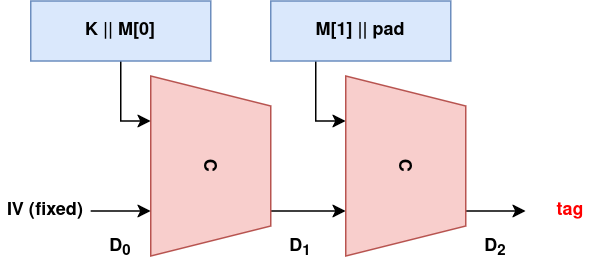
\includegraphics[width=0.45\textwidth]{img/hash_md.png}
    \par}

    È la primitiva che viene utilizzata da \textit{hash function} come \textbf{md5}, \textbf{sha1}, \textbf{sha2}. Considerando la figura, vediamo che:
    \begin{itemize}[nosep]
        \item \textbf{K} è il segreto.
        \item \textbf{M[0]} e \textbf{M[1]} è pubblico.
        \item la costruzione del \textbf{pad} è pubblica.
        \item $D_2$ è pubblico (\textbf{\textit{tag}})
    \end{itemize}
    In questa circostanza l'attaccante vince se riesce a generare un \textit{tag} valido per un certo messaggio arbitrario senza conoscere la chiave \textbf{K}. Noi (come attaccante) sappiamo che il \textit{tag} è generato \textbf{H}(\textbf{key} || \textbf{message}) dove \textbf{K} è un segreto con una data lunghezza \textbf{l} fissata, noi vogliamo calcolare un certo \textit{tag'} che venga generato \textbf{H}(\textbf{key} || \textbf{message} || \textbf{message'}).
    \begin{enumerate}[nosep]
        \item Consideriamo di utilizzare la stessa \textit{hash function}, e di ripristinare il suo stato interno come, quindi ponendo come nostro \textbf{IV} il \textit{tag} generato dalla computazione legittima, ma è necessario impostare anche il punto iniziale da dove andare a calcolare il \textbf{pad'} e deve essere pari a $len(K) + len(M) + len(pad)$.
        \item Inviamo come messaggio \textbf{M || pad || M'} e come tag quello appena calcolato \textbf{\textit{tag'}}.
        \item il destinatario calcolerà \textbf{H}(\textbf{K} || \textbf{pad} || \textbf{M} || \textbf{pad} || \textbf{M'}) e produrrà lo stesso \textit{tag'} 
    \end{enumerate}
\end{boxA}

\begin{flushleft}
    \textcolor{red}{\textbf{\textit{HMAC}}}: è un MAC che viene costruito con alla base una funzione hash (alcune volte chiamato \textbf{\textit{keyed-hash function}}), è necessario che mantenga due requisiti funzionali:
    \begin{itemize}[nosep]
        \item il \textbf{MAC} deve essere sicuro fintanto che la primitiva hash su cui è costruito è \textit{collision resistance}.
        \item per molti degli scenari presi in considerazione è sufficiente una \textit{second pre-image collision resistance}
    \end{itemize}
    Viene definito come:

    {\centering
        \textbf{HMAC}(\textbf{K}, \textbf{M}) = \textcolor{blue}{\textbf{H(}}(Kp $\oplus$ opad) || \textcolor{red}{\textbf{H(}}(Kp $\oplus$ ipad) || (m)\textcolor{red}{\textbf{)}}\textcolor{blue}{\textbf{)}}
    \par}
    Dove: 
    \begin{itemize}[nosep]
        \item \textbf{K} è un segreto a lunghezza variabile, mentre \textbf{Kp} è la sua versione \textit{zero-padded}.
        \item \textbf{opad}(\textbf{\textit{outer padding}}) e \textbf{ipad}(\textbf{\textit{inner padding}}) sono costanti con un elevata distanza di Hamming (ovvero che le posizioni di bit diversi sono elevate), utilizzate per consentire alle due funzioni hash di utilizzare chiavi diverse.
    \end{itemize}
\end{flushleft}

\begin{flushleft}
    Andiamo a considerare i \textbf{MAC} costruiti su \textit{block cipher}, il primo e il più semplice per costruire un \textbf{MAC} basato su \textit{block cipher} fu quello di utilizzare la \textbf{CBC} \textit{mode of operation} e utilizzare come \textit{tag} il testo cifrato dell'ultimo blocco.

    {\centering
        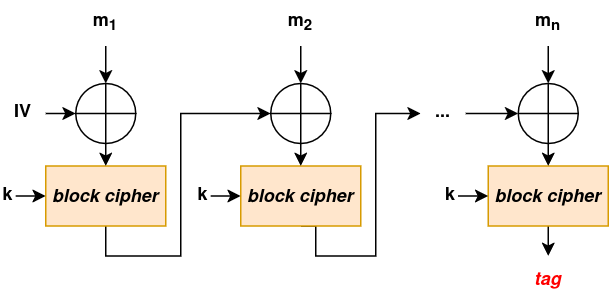
\includegraphics[width=0.45\textwidth]{img/cbc_mac.png}
    \par}

    È possibile \textit{forgiare} un messaggio, da parte di un attaccante, infatti dato \textbf{(m, t)} e \textbf{(m', t')}, un \textcolor{red}{\textbf{CBC-MAC}} producerà \textbf{t'} per un messaggio costruito come: \textbf{m || t $\oplus$ m' || m'}.

    \medskip
    
    \textcolor{red}{\textbf{\textit{CMAC}}} è il successore del \textbf{CBC-MAC} utilizza come primitiva \textbf{AES-SIV}(\textbf{CTR-CMAC}), lo schema è molto simile ma aggiunge due operazioni sull'ultimo blocco prima di utilizzarlo. Lo schema deriva due chiavi $k_1$ e $k_2$ dalla chiave originale e una delle due viene \textit{xorata} con l'ultimo blocco del messaggio $m_n$ (\textbf{\textit{tweak block}}) prima di utilizzare il blocco del \textbf{CMAC}.

    {\centering
        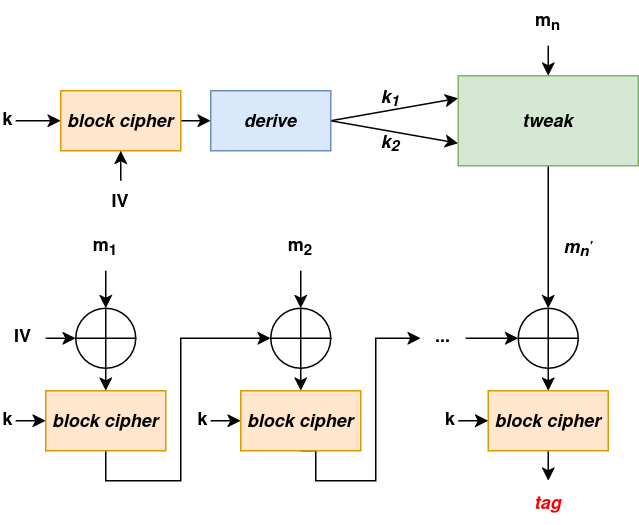
\includegraphics[width=0.45\textwidth]{img/cmac.png}
    \par}

    \newpage

    \textcolor{red}{\textbf{\textit{UHF - Universal Hash Function}}} si riferisce ad una \textbf{\textit{keyed hash function}} che prende due input: una chiave \textbf{k} e un messaggio \textbf{m}. Questa funzione garantisce che la probabilità - che dati due messaggi distinti $m_1$ e $m_2$ - di avere $UHF(m_1) = UHF(m_2)$ è \textbf{trascurabile}. Un'implementazione popolare per una funzione \textbf{UHF} è quella basata su \textbf{polinomi modulo p} (con \textbf{p} primo):
    \begin{itemize}[nosep]
        \item scegliamo un primo \textbf{p}
        \item consideriamo il messaggio $m$ come un vettore di interi in $\mathbb{Z}_p$ con un massimo di $n$ elementi: $m = [m_1, m_2, ..., m_n]$
        \item la funzione hash \textbf{H} viene calcolata utilizzando gli elementi di $m$ come coefficienti del polinomio $F(k)$:
        
        {\centering
            $H(k, M) = \overset{n}{\underset{i=1}{\sum}} (m_i \cdot k^i) \mod p$
        \par}

    \end{itemize}

    \medskip
    
    \textcolor{red}{\textbf{\textit{One-Message Polynomial evaluation MACs}}}: è possibile costruire un \textbf{MAC} partendo da delle \textbf{UHF}, consideriamo il messaggio $m = m_1, m_2, ..., m_n$

    {\centering
        $mac(m, k, r) = r + H(m, k) = r + \overset{n}{\underset{i=1}{\sum}} (m_i \cdot k^i) \mod p$
    \par}

    In questo caso il \textbf{MAC} è un polinomio di grado $n$, \textbf{p} è fissato ed è pubblico, se $m_i$ è 128bit allora $p > 128$. \textbf{k} e \textbf{r} vengono scelti randomicamente:
    \begin{itemize}[nosep]
        \item \textbf{k} lavora come la chiave per la computazione, può essere utilizzata per più messaggi.
        \item \textbf{r} ha la stessa funzionalità di un \textbf{\textit{nonce}} random, e bisogna utilizzarlo assolutamente per un unico messaggio, in questo caso \textbf{r} è \textbf{segreto}.
    \end{itemize}
    Nel caso in cui \textbf{r} venisse ripetuto per due \textit{tag}:
    \begin{align*}
        \mathbf{t_1} &= mac(m_1, k, r) = r + H(m_1, k) \\
        t_1 - r - H(m_1, k) &= 0 \\
        \mathbf{t_2} &= mac(m_2, k, r) = r + H(m_2, k) \\
        t_2 - r - H(m_2, k) &= 0
    \end{align*}

    \begin{align*}
        t_1 - \cancel{r} - H(m_1, k) &= t_2 - \cancel{r} - H(m_2, k) \\
        \overset{n}{\underset{i=1}{\sum}}(m_{1,i} \cdot k^i) + t_1 &= t_2 + \overset{n}{\underset{i=1}{\sum}}(m_{2,i} \cdot k^i) \\
        \overset{n}{\underset{i=1}{\sum}}((m_{1, i} - m_{2, i}) \cdot k^i) + t_1 - t_2 &= 0 \mod p
    \end{align*}
    In questo modo la chiave \textbf{k} è tra le radici del polinomio $m_2 - m_1 + t_1 + t_2$. 
    \smallskip
    È possibile estendere \textit{one-message poly MACs} ad un \textit{multi-message} utilizzando o una \textbf{PRF} oppure \textbf{PRP} (ad esempio un \textit{block cipher}), in questo modo, invece che utilizzare un valore di \textbf{r} random possiamo calcolarlo partendo da una chiave e un \textit{nonce}:

    {\centering
        $mac(m, k = \langle k_1, k_2 \rangle, n) = AES(n, k_1) + H(m, k_2)$
    \par}

    Se $k_1$ è segreta, un avversario, non sarebbe in grado di calcolarsi \textbf{AES}(n, $k_1$) anche se il valore $n$ fosse pubblico e non randomico, ma utilizzare lo stesso \textit{nonce} più volte esporrebbe $k_2$ e quindi romperebbe lo schema.

    \medskip

    \textcolor{red}{\textbf{\textit{GMAC}}} è basato su \textbf{AES-GCM} e in questo caso i rischi per la sicurezza in caso di errori di utilizzo sono molto più elevati a causa del comportamento lineare della funzione. Richiede un \textbf{\textit{unpredictable nonce}}, riutilizzare lo stesso \textit{nonce} per firmare messaggi diversi permette la \textbf{\textit{key recovery}}, in questo caso è molto importante utilizzare la variante \textbf{SIV} - molto più robusti a discapito delle \textit{performance} - come primivita dello schema (\textbf{AES-GCM-SIV}). La probabilità di successo in caso di attacco \textbf{aumenta} all'\textbf{aumentare della dimensione del messaggio}.

    \smallskip

    Non possiamo effettuare un'analisi a \textit{black-box} per definire come la dimensione del \textit{tag} influenzi il \textbf{livello di sicurezza}. Il dimensionamento richiede la conoscenza dello schema e le analisi sono parecchio complesse. Alcuni esempi:
    \begin{itemize}[nosep]
        \item \textbf{HMAC} e \textbf{CMAC}: è possibile mandare un numero di messaggi pari alla radice quadrata della dimensione del \textit{digest}
        \item \textbf{GHASH} (e \textbf{GMAC}): il numero dei messaggi è lineare con la dimensione del \textit{digest}, ma diminuisce rispetto alla dimensione di ogni messaggio.
        \item \textbf{Poly1305}: rappresenta un \textit{trade-off}, alto numero di messaggi dimensionalmente limitati.
    \end{itemize}
\end{flushleft}